\section{Auswertung}
\label{sec:Auswertung}
In diesem Kapitel wird der Absorptionskoeffizient von Zink und Blei ermittelt, die sich vor einer Gamma-Strahlungsquelle befinden. Im Anschluss
wird die Maximalenergie des verwendetem Beta-Strahlers bestimmt.

subsection{Bestimmung der Absorptionskoeffizienten von Blei und Eisen}
Bevor die Absorptionskoeffizienten berechnet werden können, muss von den Messwerten die Nullmessung abgezogen werden. Da hierbei nur geringe Zählraten
aufgenommen werden, wird für die Messung ein Zeitintervall von:
\begin{align*}
\Delta t = 900\,\si{\second}
\end{align*}
verwendet. Die Anzahl der Counts $N$ und die radioaktive Aktivität $A_0$ sind dann:
\begin{align*}
N &= (\num{1059 +- 33}) \\
A_0 &= (\num{1,18 +- 0,04})\,\frac{1}{\si{\second}}.
\end{align*}
Der statistische Fehler nach der Poissonverteilung von $N$ ist:
\begin{align*}
  \Delta N = \sqrt{N}.
\end{align*}
Somit wurde zur Berechnung der Aktivität folgende Fehlerformel nach der Gauß'schen Fehlerfortpflanzung verwendet:
\begin{equation}
\Delta A_0 = \frac{1}{\Delta t} \cdot \sqrt{N}.
\end{equation}
Nun wird der Absorptionskoeffizient von Blei mit Hilfe einer Ausgleichsrechnung bestimmt. Dazu wird die Aktivität gegen die Dicke des zu durchdringenden Materials
in einem halblogarithmischen Diagram aufgetragen. Nach Gleichung (2) besteht zwischen der Aktivität und der Dicke des Materials ein exponentieller
Zusammenhang. Durch Umstellen und Logarithmieren dieser Gleichung wird folgender Zusammenhang deutlich:
\begin{align*}
\ln{A(D)} = - \mu \cdot D + \ln{A_0}.
\end{align*}
Dies lässt nun auf eine lineare Ausgleichsrechnung deuten, welche folgende Form hat:
\begin{equation}
\label{eqn:ausgleich1}
A(D) = - a \cdot D + b.
\end{equation}
Die für die lineare Regression verwendeten Messwerte befinden sich in Tabelle \ref{tab:blei} und der Graph ist in Abbildung \ref{fig:blei} zu sehen.
\begin{figure}[H]
  \center
  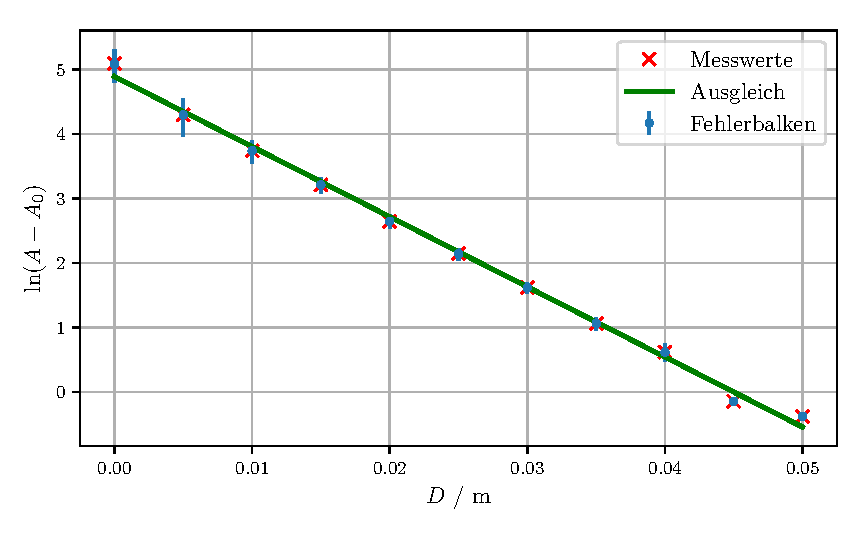
\includegraphics[scale = 0.75]{blei.pdf}
  \caption{Lineare Regression zur Bestimmung des Absorptionskoeffizienten von Blei.}
  \label{fig:blei}
\end{figure}
\begin{table}[H]
  \centering
  \caption{Messwerte zur Bestimmung des Absorptionskoeffizienten von Blei.}
  \label{tab:blei}
  \begin{tabular}{c c c c c}
    \toprule
$D\:/\:\si{\meter}$ & $t\:/\:\si{\second}$ & Counts $N$ & $A\:/\:\frac{1}{\si{\second}}$ & $(A-A_0)\:/\:\frac{1}{\si{\second}}$ \\
    \midrule
    0.00  & 100 & \num{16308 +- 128} & \num{163.08 +- 1.28}   & \num{162.06 +- 1.28} \\
    0.005 & 50  & \num{3722 +- 61}   & \num{74.44 +- 1.22}    & \num{73.42 +- 1.22}  \\
    0.01  & 100 & \num{4320 +- 66}   & \num{43.20 +- 0.66}    & \num{42.18 +- 0.66}  \\
    0.015 & 150 & \num{3870 +- 62}   & \num{25.80 +- 0.41}    & \num{24.78  +- 0.41} \\
    0.02  & 200 & \num{3024 +- 55}   & \num{15.12 +- 0.27}    & \num{14.10  +- 0.27} \\
    0.025 & 250 & \num{2384 +- 49}   & \num{9.54 +- 0.20}     & \num{8.52 +- 0.20}  \\
    0.03  & 300 & \num{1814 +- 43}   & \num{6.05 +- 0.14}     & \num{5.03 +- 0.14}  \\
    0.035 & 400 & \num{1564 +- 40}   & \num{3.91 +- 0.10}     & \num{2.89 +- 0.10}  \\
    0.04  & 500 & \num{1435 +- 38}   & \num{2.87 +- 0.08}     & \num{1.85 +- 0.08}  \\
    0.045 & 500 & \num{942 +- 31}    & \num{1.88 +- 0.06}     & \num{0.86 +- 0.06}  \\
    0.05  & 500 & \num{853 +- 29}    & \num{1.71 +- 0.06}     & \num{0.69 +- 0.06}  \\
    \bottomrule
  \end{tabular}
\end{table}
\noindent Die nach Gleichung \eqref{eqn:ausgleich1} berechneten Parameter $a$ und $b$ entsprechen dem Absorptionskoeffizienten und der Anfangsaktivität und sind somit:
\begin{align*}
a &= \mu = (\num{108.7 +- 2.1})\,\frac{1}{\si{\meter}} \\
b &= A_\text{A} = (\num{133 +- 8})\,\frac{1}{\si{\second}}.
\end{align*}
Der theoretische Wert für den Compton-Absorptionskoeffizienten lässt sich mit Hilfe der Gleichung (6) berechnen.
Die für diese Berechnung benötigten Werte sind folgende:
\begin{align*}
\epsilon &= 1,295 \: \text{\cite[S.243]{kent}} ,\\
r_e &= 2,82 \cdot 10^{-15}\,\si{\meter} \: \text{\cite[S.235]{kent}} ,\\
N_\text{A} &= 6,022 \cdot 10^{23} \,\frac{1}{\si{\mol}} \text{\cite{kent4}},\\
\rho &= 11342\,\frac{\si{\kilo\gram}}{\si{\cubic\meter}} \: \text{\cite{kent2}},\\
Z &= 82 ,\\
M &= 207,2\,\frac{\si{\gram}}{\si{\mol}} \: \text{\cite{kent3}}.
\end{align*}
Daraus ergibt sich nun der Compton-Absorptionskoeffizient:
\begin{align*}
  \mu_{com, \text{Pb}} = 69,35\,\frac{1}{\si{\meter}}.
\end{align*}

\noindent Nun wird analog der Absorptionskoeffizent von Eisen ermittelt. Die hierfür benötigten Messwerte befinden sich in Tabelle \ref{tab:eisen}
und die lineare Regression nach Gleichung \eqref{eqn:ausgleich1} befindet sich in Abbildung \ref{fig:eisen}.
%EISEN
\begin{figure}[H]
  \center
  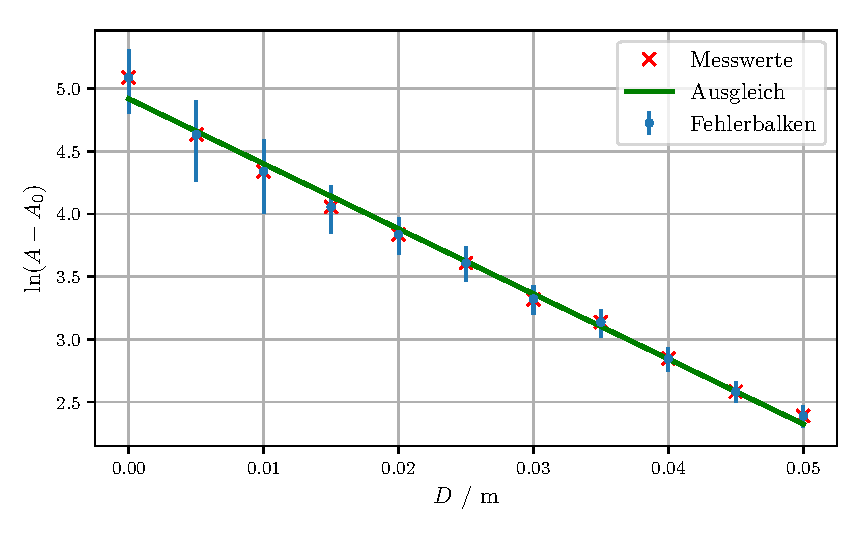
\includegraphics[scale = 0.75]{eisen.pdf}
  \caption{Lineare Regression zur Bestimmung des Absorptionskoeffizienten von Blei.}
  \label{fig:eisen}
\end{figure}
\begin{table}[H]
  \centering
  \caption{Messwerte zur Bestimmung des Absorptionskoeffizienten von Blei.}
  \label{tab:eisen}
  \begin{tabular}{c c c c c}
    \toprule
$D\:/\:\si{\meter}$ & $t\:/\:\si{\second}$ & Counts $N$ & $A\:/\:\frac{1}{\si{\second}}$ & $(A-A_0)\:/\:\frac{1}{\si{\second}}$ \\
    \midrule
    0.005 & 50  & \num{5193 +- 72} & \num{103.86 +- 1.44} & \num{102.8 +- 1.44} \\
    0.01  & 50  & \num{3884 +- 62} & \num{77.68 +- 1.25} & \num{76.66 +- 1.25} \\
    0.015 & 100 & \num{5879 +- 77} & \num{58.79 +- 0.77} & \num{57.77 +- 0.77} \\
    0.02  & 150 & \num{7104 +- 84} & \num{47.36 +- 0.56} & \num{46.34 +- 0.56} \\
    0.025 & 150 & \num{5691 +- 75} & \num{37.94 +- 0.50} & \num{36.92 +- 0.50} \\
    0.03  & 200 & \num{5741 +- 76} & \num{28.71 +- 0.38} & \num{27.69 +- 0.38} \\
    0.035 & 200 & \num{4809 +- 69} & \num{24.05 +- 0.35} & \num{23.03 +- 0.35} \\
    0.04  & 250 & \num{4559 +- 68} & \num{18.24 +- 0.27} & \num{17.22 +- 0.27} \\
    0.045 & 300 & \num{4277 +- 65} & \num{14.26  +- 0.22} & \num{13.24 +- 0.22} \\
    0.05  & 300 & \num{3578 +- 60} & \num{11.93 +- 0.20} & \num{10.91 +- 0.20} \\
    \bottomrule
  \end{tabular}
\end{table}

\noindent Die nach Gleichung \eqref{eqn:ausgleich1} berechneten Parameter $a$ und $b$ entsprechen erneut dem Absorptionskoeffizienten und der Anfangsaktivität und sind somit:
\begin{align*}
a &= \mu = (\num{51.9 +- 1.4})\,\frac{1}{\si{\meter}} ,\\
b &= A_\text{A} = (\num{137 +- 6})\,\frac{1}{\si{\second}}.
\end{align*}
Der theoretische Wert für den Compton-Absorptionskoeffizienten lässt sich mit Hilfe der Gleichung (6) berechnen.
Die für diese Berechnung benötigten Werte sind folgende:
\begin{align*}
\rho &= 7874\,\frac{\si{\kilo\gram}}{\si{\cubic\meter}}\:\text{\cite{kent2}},\\
Z &= 26 ,\\
M &= 55,845\,\frac{\si{\gram}}{\si{\mol}}\: \text{\cite{kent3}}.
\end{align*}
Die Werte für $\epsilon$, dem Elektronenradius $r_e$ und der Avogadro-Konstante $N_\text{A}$ sind die selben geblieben.
Daraus ergibt sich nun der Compton-Absorptionskoeffizient:
\begin{align*}
  \mu_{com, \text{Fe}} = 56,64\,\frac{1}{\si{\meter}}.
\end{align*}

\subsection{Bestimmung der Maximalenergie der Beta-Strahlung}
Für die Bestimmung der Maximalenergie der Beta-Strahlung wird zunächst die maximale Reichweite $R_\text{max}$ der Elektronen bestimmt.
Dazu wird die Aktivität gegen die Massenbelegung aufgetragen und gemäß Abbildung \ref{fig:absorp} in zwei Teile aufgeteilt. Die einzelnen Teile
werden dann mit einer linearen Regression gefittet. Ziel ist es, die Stelle zu errechnen, an der sich beide Graphen treffen. Der $x$-Wert dieses
Schnittpunktes gibt dann die maximale Reichweite der Elektronen an. Die Ausgleichsrechnung wird analog zur Gleichung \eqref{eqn:ausgleich1} durchgeführt, wobei
die Parameter verändert wurden. Die neuen Parameter sind $A_i$ und $B_i$ mit $i=1,\: 2$. Die beiden Graphen sind in Abbildung \ref{fig:reichweite} zu sehen.
Die Massenbelegung, welche durch die Formel \eqref{eqn:masse} berechnet wird, befindet sich zusammen mit den Messwerten in Tabelle \ref{tab:reichweite}.
Dabei ist die Dichte von Aluminium
\begin{align*}
\rho = 2698\,\frac{\si{\kilo\gram}}{\si{\cubic\meter}} \text{\cite{kent2}}.
\end{align*}
\begin{figure}[H]
  \center
  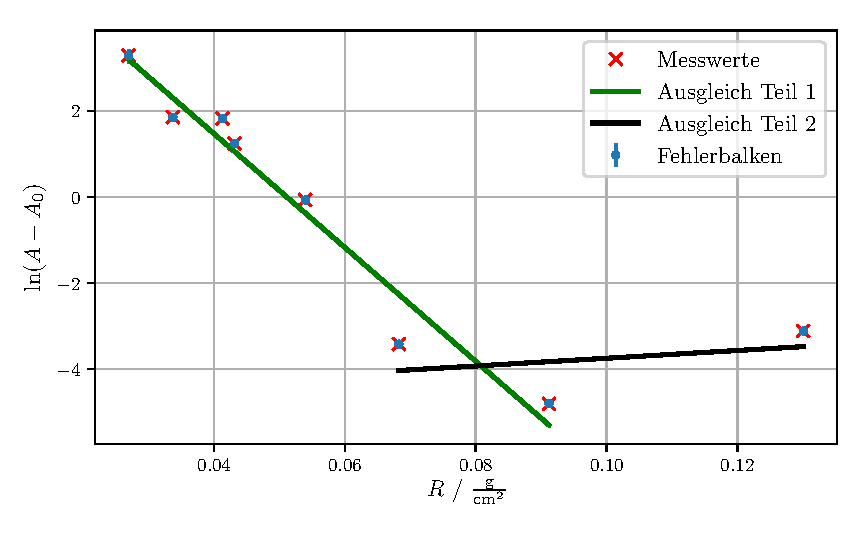
\includegraphics[scale = 0.75]{beta.pdf}
  \caption{Zwei lineare Regressionen zur Bestimmung der maximalen Reichweite $R_\text{max}$ der Beta-Strahlung.}
  \label{fig:reichweite}
\end{figure}
\begin{table}[H]
  \centering
  \caption{Messwerte zur Bestimmung der maximalen Reichweite.}
  \label{tab:reichweite}
  \begin{tabular}{c c c c c c}
    \toprule
$D\:/\:\si{\micro\meter}$ & $t\:/\:\si{\second}$ & Counts $N$ & $A\:/\:\frac{1}{\si{\second}}$ & $(A-A_0)\:/\:\frac{1}{\si{\second}}$ &
$R\:/\:\frac{\si{\gram}}{\si{\centi\meter\squared}}$ \\
    \midrule
100 & 100  & \num{2743 +- 52} & \num{27.43 +- 0.45} & \num{26.72 +- 0.47} & \num{0.027} \\
125 & 200  & \num{1418 +- 38} & \num{7.09 +- 0.22}  & \num{6.38 +- 0.22} & \num{0.034} \\
153 & 300  & \num{2064 +- 45} & \num{6.88 +- 0.22}  & \num{6.17 +- 0.22} & \num{0.04} \\
160 & 400  & \num{1673 +- 41} & \num{4.18 +- 0.14}  & \num{3.48 +- 0.14} & \num{0.04} \\
200 & 500  & \num{820 +- 29}  & \num{1.64 +- 0.07}  & \num{0.93 +- 0.07} & \num{0.05} \\
253 & 600  & \num{443 +- 21}  & \num{0.74 +- 0.04}  & \num{0.33 +- 0.04} & \num{0.07} \\
302 & 700  & \num{459 +- 21}  & \num{0.66 +- 0.04}  & \num{-0.05 +- 0.04} & \num{0.08} \\
338 & 800  & \num{571 +- 24}  & \num{0.71 +- 0.03}  & \num{0.01 +- 0.04} & \num{0.09} \\
400 & 900  & \num{583 +- 24}  & \num{0.65 +- 0.03}  & \num{-0.06 +- 0.04} & \num{0.11} \\
444 & 1000 & \num{689 +- 26}  & \num{0.68 +- 0.03}  & \num{-0.02 +- 0.04} & \num{0.12} \\
482 & 1100 & \num{825 +- 29}  & \num{0.75 +- 0.04}  & \num{0.04 +- 0.04} & \num{0.13} \\
    \bottomrule
  \end{tabular}
\end{table}
\noindent Die Parameter sind $A_i$ und $B_i$ sind nach Gleichung \eqref{eqn:ausgleich1} folgende:
%SO WAR ES VORHER / VON ROMAN:
%A_1 &= (\num{132 +- 12})\,\frac{\si{\centi\meter\squared}}{\si{\gram}} \\
%B_1 &= (\num{680 +- 70})\,\frac{1}{\si{\second}}, \\
%\intertext{und} \\
%A_2 &= (\num{0.9 +- 2.7})\,\frac{\si{\centi\meter\squared}}{\si{\gram}} \\
%B_2 &= (\num{4.6 +- 2.7})\,\frac{1}{\si{\second}}.
\begin{align*}
A_1 &= (\num{-132 +- 12})\,\frac{\si{\centi\meter\squared}}{\si{\gram}} ,\\
B_1 &= (\num{6.8 +- 0.7})\,\frac{1}{\si{\second}} \\
\intertext{und} \\
A_2 &= (\num{9 +- 27})\,\frac{\si{\centi\meter\squared}}{\si{\gram}} ,\\
B_2 &= (\num{-4.6 +- 2.7})\,\frac{1}{\si{\second}}.
\end{align*}
Die maximale Reichweite, also der Schnittpunkt dieser beiden Geraden wird folgendermaßen berechnet:
\begin{equation}
  \label{eqn:reichweite}
R_\text{max} = \frac{B_1 \cdot 1\,\si{\second} - B_2 \cdot 1\,\si{\second}}{A_2 - A_1}
\end{equation}
Der Fehler ist dann nach der Gauß'schen Fehlerfortpflanzung so definiert:
\begin{equation}
  \tiny
\label{eqn:reichweitef}
\Delta R_\text{max} = \sqrt{\left(- \ln{\left (B_{1} \right )} +
\ln{\left (B_{2} \right )}\right)^{2} \left( \frac{\Delta{A_{1}}^{2}}{\left(A_{1} - A_{2}\right)^{4}} + \frac{\Delta{A_{2}}^{2}}{\left(A_{1} - A_{2}\right)^{4}} \right)
 + \frac{\Delta{B_{2}}^{2}}{B_{2}^{2}
\left(A_{1} - A_{2}\right)^{2}} + \frac{\Delta{B_{1}}^{2}}{B_{1}^{2} \left(A_{1} - A_{2}\right)^{2}}}
\end{equation}
Nach Gleichung \eqref{eqn:reichweite} und \eqref{eqn:reichweitef} ergibt sich für die maximale Reichweite:
\begin{align*}
R_\text{max} = (\num{0.081 +- 0.026})\,\frac{\si{\gram}}{\si{\centi\meter\squared}}.
\end{align*}
Mit dieser Reichweite lässt sich nun nach Gleichung \eqref{eqn:emax} die maximale Energie ausrechnen:
\begin{align*}
E_\text{max} = (\num{0.30 +- 0.06})\,\si{\mega\electronvolt}.
\end{align*}
Der Fehler der maximalen Energie lässt sich mit Hilfe folgender Gleichung bestimmen:
\begin{equation}
\Delta E_\text{max} = 1.92 \cdot \frac{\Delta R_\text{max} \left(R_\text{max} + 0.11\right)}{\sqrt{R_\text{max}^{2} + 0.22 R_\text{max}}}.
\end{equation}
